\documentclass[]{article}
\usepackage{lmodern}
\usepackage{amssymb,amsmath}
\usepackage{ifxetex,ifluatex}
\usepackage{fixltx2e} % provides \textsubscript
\ifnum 0\ifxetex 1\fi\ifluatex 1\fi=0 % if pdftex
  \usepackage[T1]{fontenc}
  \usepackage[utf8]{inputenc}
\else % if luatex or xelatex
  \ifxetex
    \usepackage{mathspec}
  \else
    \usepackage{fontspec}
  \fi
  \defaultfontfeatures{Ligatures=TeX,Scale=MatchLowercase}
\fi
% use upquote if available, for straight quotes in verbatim environments
\IfFileExists{upquote.sty}{\usepackage{upquote}}{}
% use microtype if available
\IfFileExists{microtype.sty}{%
\usepackage{microtype}
\UseMicrotypeSet[protrusion]{basicmath} % disable protrusion for tt fonts
}{}
\usepackage[margin=1in]{geometry}
\usepackage{hyperref}
\hypersetup{unicode=true,
            pdftitle={5 Parameter estimation and model identification for ARMA models},
            pdfauthor={Edward Ionides},
            pdfborder={0 0 0},
            breaklinks=true}
\urlstyle{same}  % don't use monospace font for urls
\usepackage{color}
\usepackage{fancyvrb}
\newcommand{\VerbBar}{|}
\newcommand{\VERB}{\Verb[commandchars=\\\{\}]}
\DefineVerbatimEnvironment{Highlighting}{Verbatim}{commandchars=\\\{\}}
% Add ',fontsize=\small' for more characters per line
\usepackage{framed}
\definecolor{shadecolor}{RGB}{248,248,248}
\newenvironment{Shaded}{\begin{snugshade}}{\end{snugshade}}
\newcommand{\KeywordTok}[1]{\textcolor[rgb]{0.13,0.29,0.53}{\textbf{#1}}}
\newcommand{\DataTypeTok}[1]{\textcolor[rgb]{0.13,0.29,0.53}{#1}}
\newcommand{\DecValTok}[1]{\textcolor[rgb]{0.00,0.00,0.81}{#1}}
\newcommand{\BaseNTok}[1]{\textcolor[rgb]{0.00,0.00,0.81}{#1}}
\newcommand{\FloatTok}[1]{\textcolor[rgb]{0.00,0.00,0.81}{#1}}
\newcommand{\ConstantTok}[1]{\textcolor[rgb]{0.00,0.00,0.00}{#1}}
\newcommand{\CharTok}[1]{\textcolor[rgb]{0.31,0.60,0.02}{#1}}
\newcommand{\SpecialCharTok}[1]{\textcolor[rgb]{0.00,0.00,0.00}{#1}}
\newcommand{\StringTok}[1]{\textcolor[rgb]{0.31,0.60,0.02}{#1}}
\newcommand{\VerbatimStringTok}[1]{\textcolor[rgb]{0.31,0.60,0.02}{#1}}
\newcommand{\SpecialStringTok}[1]{\textcolor[rgb]{0.31,0.60,0.02}{#1}}
\newcommand{\ImportTok}[1]{#1}
\newcommand{\CommentTok}[1]{\textcolor[rgb]{0.56,0.35,0.01}{\textit{#1}}}
\newcommand{\DocumentationTok}[1]{\textcolor[rgb]{0.56,0.35,0.01}{\textbf{\textit{#1}}}}
\newcommand{\AnnotationTok}[1]{\textcolor[rgb]{0.56,0.35,0.01}{\textbf{\textit{#1}}}}
\newcommand{\CommentVarTok}[1]{\textcolor[rgb]{0.56,0.35,0.01}{\textbf{\textit{#1}}}}
\newcommand{\OtherTok}[1]{\textcolor[rgb]{0.56,0.35,0.01}{#1}}
\newcommand{\FunctionTok}[1]{\textcolor[rgb]{0.00,0.00,0.00}{#1}}
\newcommand{\VariableTok}[1]{\textcolor[rgb]{0.00,0.00,0.00}{#1}}
\newcommand{\ControlFlowTok}[1]{\textcolor[rgb]{0.13,0.29,0.53}{\textbf{#1}}}
\newcommand{\OperatorTok}[1]{\textcolor[rgb]{0.81,0.36,0.00}{\textbf{#1}}}
\newcommand{\BuiltInTok}[1]{#1}
\newcommand{\ExtensionTok}[1]{#1}
\newcommand{\PreprocessorTok}[1]{\textcolor[rgb]{0.56,0.35,0.01}{\textit{#1}}}
\newcommand{\AttributeTok}[1]{\textcolor[rgb]{0.77,0.63,0.00}{#1}}
\newcommand{\RegionMarkerTok}[1]{#1}
\newcommand{\InformationTok}[1]{\textcolor[rgb]{0.56,0.35,0.01}{\textbf{\textit{#1}}}}
\newcommand{\WarningTok}[1]{\textcolor[rgb]{0.56,0.35,0.01}{\textbf{\textit{#1}}}}
\newcommand{\AlertTok}[1]{\textcolor[rgb]{0.94,0.16,0.16}{#1}}
\newcommand{\ErrorTok}[1]{\textcolor[rgb]{0.64,0.00,0.00}{\textbf{#1}}}
\newcommand{\NormalTok}[1]{#1}
\usepackage{longtable,booktabs}
\usepackage{graphicx,grffile}
\makeatletter
\def\maxwidth{\ifdim\Gin@nat@width>\linewidth\linewidth\else\Gin@nat@width\fi}
\def\maxheight{\ifdim\Gin@nat@height>\textheight\textheight\else\Gin@nat@height\fi}
\makeatother
% Scale images if necessary, so that they will not overflow the page
% margins by default, and it is still possible to overwrite the defaults
% using explicit options in \includegraphics[width, height, ...]{}
\setkeys{Gin}{width=\maxwidth,height=\maxheight,keepaspectratio}
\IfFileExists{parskip.sty}{%
\usepackage{parskip}
}{% else
\setlength{\parindent}{0pt}
\setlength{\parskip}{6pt plus 2pt minus 1pt}
}
\setlength{\emergencystretch}{3em}  % prevent overfull lines
\providecommand{\tightlist}{%
  \setlength{\itemsep}{0pt}\setlength{\parskip}{0pt}}
\setcounter{secnumdepth}{0}
% Redefines (sub)paragraphs to behave more like sections
\ifx\paragraph\undefined\else
\let\oldparagraph\paragraph
\renewcommand{\paragraph}[1]{\oldparagraph{#1}\mbox{}}
\fi
\ifx\subparagraph\undefined\else
\let\oldsubparagraph\subparagraph
\renewcommand{\subparagraph}[1]{\oldsubparagraph{#1}\mbox{}}
\fi

%%% Use protect on footnotes to avoid problems with footnotes in titles
\let\rmarkdownfootnote\footnote%
\def\footnote{\protect\rmarkdownfootnote}

%%% Change title format to be more compact
\usepackage{titling}

% Create subtitle command for use in maketitle
\newcommand{\subtitle}[1]{
  \posttitle{
    \begin{center}\large#1\end{center}
    }
}

\setlength{\droptitle}{-2em}
  \title{5 Parameter estimation and model identification for ARMA models}
  \pretitle{\vspace{\droptitle}\centering\huge}
  \posttitle{\par}
  \author{Edward Ionides}
  \preauthor{\centering\large\emph}
  \postauthor{\par}
  \predate{\centering\large\emph}
  \postdate{\par}
  \date{2018-01-23}


\begin{document}
\maketitle

{
\setcounter{tocdepth}{2}
\tableofcontents
}
\newcommand\prob{\mathbb{P}}
\newcommand\E{\mathbb{E}}
\newcommand\var{\mathrm{Var}}
\newcommand\cov{\mathrm{Cov}}
\newcommand\loglik{\ell}
\newcommand\R{\mathbb{R}}
\newcommand\data[1]{#1^*}
\newcommand\estimate[1]{\data{#1}}
\newcommand\params{\, ; \,}
\newcommand\transpose{\scriptsize{T}}
\newcommand\eqspace{\quad\quad\quad}
\newcommand\lik{\mathcal{L}}
\newcommand\profileloglik[1]{\ell^\mathrm{profile}_#1}
\newcommand\ar{\phi}
\newcommand\ma{\psi}




\begin{center}\rule{0.5\linewidth}{\linethickness}\end{center}

\begin{center}\rule{0.5\linewidth}{\linethickness}\end{center}

Objectives

\begin{enumerate}
\def\labelenumi{\arabic{enumi}.}
\item
  Develop likelihood-based inference in the context of ARMA models.
\item
  Discuss maximum likelihood parameter estimation and alternative
  methods.
\item
  Investigate strategies for model selection, also known as model
  identification, in the context of ARMA models.
\item
  Work on practical computational approaches for implementing these
  methods.
\end{enumerate}

\begin{center}\rule{0.5\linewidth}{\linethickness}\end{center}

\begin{center}\rule{0.5\linewidth}{\linethickness}\end{center}

\subsection{Background on likelihood-based
inference}\label{background-on-likelihood-based-inference}

\begin{itemize}
\item
  For any data \(\data{y_{1:N}}\) and any probabilistic model
  \(f_{Y_{1:N}}(y_{1:N}\params\theta)\) we define the likelihood
  function to be
  \[ \lik(\theta) = f_{Y_{1:N}}(\data{y_{1:N}}\params\theta).\]
\item
  It is often convenient to work with the logarithm to base \(e\) of the
  likelihood, which we write as \[\loglik(\theta) = \log \lik(\theta).\]
\item
  Using the likelihood function as a statistical tool is a very general
  technique, widely used since
  \href{https://en.wikipedia.org/wiki/Likelihood_function}{Fisher
  (1922)}.
\item
  Time series analysis involves various situations where we can, with
  sufficient care, compute the likelihood function and take advantage of
  the general framework of likelihood-based inference.
\item
  Computation of the likelihood function for ARMA models is not entirely
  straightforward.

  \begin{itemize}
  \item
    Computationally efficient algorithms exist, using a state space
    model representation of ARMA models that will be developed later in
    this course.
  \item
    For now, it is enough that software exists to evaluate and maximize
    the likelihood function for a Gaussian ARMA model. Our immediate
    task is to think about how to use that capability.
  \end{itemize}
\item
  Before evaluation of the ARMA likelihood became routine, it was
  popular to use a method of moments estimator called
  \textbf{Yule-Walker} estimation. This is described by Shumway and
  Stoffer (Section 3.6) but is nowadays mostly of historical interest.
\item
  There are occasionally time series situations where massively long
  data or massively complex models mean that it is computationally
  infeasible to work with the likelihood function. However, we are going
  to focus on the common situation where we can (with due care) work
  with the likelihood.
\item
  Likelihood-based inference (meaning statistical tools based on the
  likelihood function) provides tools for parameter estimation, standard
  errors, hypothesis tests and diagnosing model misspecification.
\item
  Likelihood-based inference often (but not always) has favorable
  theoretical properties. Here, we are not especially concerned with the
  underlying theory of likelihood-based inference. On any practical
  problem, we can check the properties of a statistical procedure by
  simulation experiments.
\end{itemize}

\subsection{The maximum likelihood estimator
(MLE)}\label{the-maximum-likelihood-estimator-mle}

\begin{itemize}
\item
  A maximum likelihood estimator (MLE) is
  \[ \hat\theta(y_{1:N}) = \arg\max_\theta f_{Y_{1:N}}(y_{1:N}\params\theta),\]
  where \(\arg\max_\theta g(\theta)\) means a value of argument
  \(\theta\) at which the maximum of the function \(g\) is attained, so
  \(g\big(\arg\max_\theta g(\theta)\big) = \max_\theta g(\theta)\).
\item
  If there are many values of \(\theta\) giving the same maximum value
  of the likelihood, then an MLE still exists but is not unique.
\item
  The maximum likelihood estimate (also known as the MLE) is

  \begin{eqnarray} \estimate{\hat\theta} &=& \hat\theta(\data{y_{1:N}})
  \\
  &=& \arg\max_\theta \lik(\theta)
  \\
  &=& \arg\max_\theta \loglik(\theta).
  \end{eqnarray}
\end{itemize}

\begin{center}\rule{0.5\linewidth}{\linethickness}\end{center}

\begin{center}\rule{0.5\linewidth}{\linethickness}\end{center}

\subsubsection{\texorpdfstring{Question: Why are
\(\arg\max_\theta \lik(\theta)\) and \(\arg\max_\theta \loglik(\theta)\)
the
same?}{Question: Why are \textbackslash{}arg\textbackslash{}max\_\textbackslash{}theta \textbackslash{}lik(\textbackslash{}theta) and \textbackslash{}arg\textbackslash{}max\_\textbackslash{}theta \textbackslash{}loglik(\textbackslash{}theta) the same?}}\label{question-why-are-argmax_theta-liktheta-and-argmax_theta-logliktheta-the-same}

\begin{center}\rule{0.5\linewidth}{\linethickness}\end{center}

\begin{center}\rule{0.5\linewidth}{\linethickness}\end{center}

\begin{itemize}
\tightlist
\item
  We can write \(\hat\theta_{MLE}\) and \(\estimate{\hat\theta_{MLE}}\)
  if we are considering various alternative estimation methods. However,
  in this course, we will most often be using maximum likelihood
  estimation so we let \(\hat\theta\) and \(\estimate{\hat\theta}\)
  correspond to this approach.
\end{itemize}

\begin{center}\rule{0.5\linewidth}{\linethickness}\end{center}

\begin{center}\rule{0.5\linewidth}{\linethickness}\end{center}

\subsection{Standard errors for the
MLE}\label{standard-errors-for-the-mle}

\begin{itemize}
\item
  As statisticians, it would be irresponsible to present an estimate
  without a measure of uncertainty!
\item
  Usually, this means obtaining a confidence interval, or an approximate
  confidence interval.

  \begin{itemize}
  \item
    It is good to say \textbf{approximate} when you present something
    that is not exactly a confidence interval with the claimed coverage.
    For example, remind yourself of the definition of a 95\% confidence
    interval.
  \item
    Saying ``approximate'' reminds you that there is some checking that
    could be done to assess how accurate the approximation is in your
    particular situation.
  \item
    It also helps to remind you that it may be interesting and relevant
    to explain why the interval you present is an approximate confidence
    interval rather than an exact one.
  \end{itemize}
\item
  There are three main approaches to estimating the statistical
  uncertainty in an MLE.
\end{itemize}

\begin{enumerate}
\def\labelenumi{\arabic{enumi}.}
\item
  The Fisher information. This is computationally quick, but works well
  only when \(\hat\theta(Y_{1:N})\) is well approximated by a normal
  distribution.
\item
  Profile likelihood estimation. This is a bit more computational
  effort, but generally is preferable to the Fisher information.
\item
  A simulation study, also known as a bootstrap.

  \begin{itemize}
  \item
    If done carefully and well, this can be the best approach.
  \item
    A confidence interval is a claim about reproducibility. You claim,
    so far as your model is correct, that on 95\% of realizations from
    the model, a 95\% confidence interval you have constructed will
    cover the true value of the parameter.
  \item
    A simulation study can check this claim fairly directly, but
    requires the most effort.
  \item
    The simulation study takes time for you to develop and debug, time
    for you to explain, and time for the reader to understand and check
    what you have done. We usually carry out simulation studies to check
    our main conclusions only.
  \end{itemize}
\end{enumerate}

\begin{center}\rule{0.5\linewidth}{\linethickness}\end{center}

\begin{center}\rule{0.5\linewidth}{\linethickness}\end{center}

\subsubsection{Standard errors via the observed Fisher
information}\label{standard-errors-via-the-observed-fisher-information}

\begin{itemize}
\item
  We suppose that \(\theta\in\R^D\) and so we can write
  \(\theta=\theta_{1:D}\).
\item
  The \href{https://en.wikipedia.org/wiki/Hessian_matrix}{Hessian
  matrix} of a function is the matrix of its second partial derivatives.
  We write the Hessian matrix of the log likelihood function as
  \(\nabla^2\loglik(\theta)\), a \(D\times D\) matrix whose \((i,j)\)
  element is
  \[ \big[\nabla^2\loglik(\theta)\big]_{ij} =  \frac{\partial^2}{\partial\theta_i\partial\theta_j}\loglik(\theta).\]
\item
  The observed Fisher information is
  \[ \estimate{\hat{I}} = - \nabla^2\loglik(\estimate{\hat\theta}).\]
\item
  A standard asymptotic approximation to the distribution of the MLE for
  large \(N\) is \[
  \hat\theta(Y_{1:N}) \approx N\left[\theta, [\estimate{\hat{I}}]^{-1}\right],
  \] where \(\theta\) is the true parameter value. This asserts that the
  MLE is asymptotically unbiased, with variance asymptotically attaining
  the Cramer-Rao lower bound. Thus, we say the MLE is
  \textbf{asymptotically efficient}. Here, we interpret \(\approx\) to
  mean ``one could write a limit statement formally justifying this
  approximation in a suitable limit.''
\item
  A corresponding approximate 95\% confidence interval for \(\theta_d\)
  is
  \[ \estimate{\hat\theta_d} \pm 1.96 \big[({\estimate{\hat{I}}})^{-1}\big]_{dd}^{1/2}.\]
\item
  The R function \texttt{arima} computes standard errors for the MLE of
  an ARMA model in this way.
\item
  We usually only have one time series, with some fixed \(N\), and so we
  cannot in practice take \(N\to\infty\). When our time series model is
  non-stationary it may not even be clear what it would mean to take
  \(N\to\infty\). These asymptotic results should be viewed as nice
  mathematical reasons to consider computing an MLE, but not a
  substitute for checking how the MLE behaves for our model and data.
\end{itemize}

\begin{center}\rule{0.5\linewidth}{\linethickness}\end{center}

\subsubsection{Confidence intervals via the profile
likelihood}\label{confidence-intervals-via-the-profile-likelihood}

\begin{itemize}
\item
  Let's consider the problem of obtaining a confidence interval for
  \(\theta_d\), the \(d\)th component of \(\theta_{1:D}\).
\item
  The \textbf{profile log likelihood function} of \(\theta_d\) is
  defined to be
  \[ \profileloglik{d}(\theta_d) = \max_{\phi\in\R^D: \phi_d=\theta_d}\loglik(\phi).\]
  In general, the profile likelihood of one parameter is constructed by
  maximizing the likelihood function over all other parameters.
\item
  Check that
  \(\max_{\theta_d}\profileloglik{d}(\theta_d) = \max_{\theta_{1:D}}\loglik(\theta_{1:D})\).
  Maximizing the profile likelihood \(\profileloglik{d}(\theta_d)\)
  gives the MLE, \(\estimate{\hat\theta_d}\).
\item
  An approximate 95\% confidence interval for \(\theta_d\) is given by
  \[ \big\{\theta_d : \loglik(\estimate{\hat\theta}) - \profileloglik{d}(\theta_d)< 1.92\big\}.\]
\item
  This is known as a profile likelihood confidence interval. The cutoff
  \(1.92\) is derived using
  \href{https://en.wikipedia.org/wiki/Likelihood-ratio_test\#Distribution:_Wilks.27s_theorem}{Wilks's
  theorem}, which we will discuss in more detail when we develop
  likelihood ratio tests.
\item
  Although the asymptotic justification of Wilks's theorem is the same
  limit that justifies the Fisher information standard errors, profile
  likelihood confidence intervals tend to work better than Fisher
  information confidence intervals when \(N\) is not so
  large---particularly when the log likelihood function is not close to
  quadratic near its maximum.
\end{itemize}

\begin{center}\rule{0.5\linewidth}{\linethickness}\end{center}

\begin{center}\rule{0.5\linewidth}{\linethickness}\end{center}

\subsubsection{Bootstrap methods for constructing standard errors and
confidence
intervals}\label{bootstrap-methods-for-constructing-standard-errors-and-confidence-intervals}

\begin{itemize}
\item
  Suppose we want to know the statistical behavior of the estimator
  \(\hat\theta({y_{1:N}})\) for models in a neighborhood of the MLE,
  \(\data{\theta}=\hat\theta(\data{y_{1:N}})\).
\item
  In particular, let's consider the problem of estimating uncertainty
  about \(\theta_1\). We want to assess the behavior of the maximum
  likelihood estimator, \(\hat\theta({y_{1:N}})\), and possibly the
  coverage of an associated confidence interval estimator,
  \(\big[\hat\theta_{1,\mathrm lo}({y_{1:N}}),\hat\theta_{1,\mathrm hi}({y_{1:N}})\big]\).
  The confidence interval estimator could be constructed using either
  the Fisher information method or the profile likelihood approach.
\item
  The following simulation study lets us address the following goals: 
\end{itemize}

\begin{enumerate}
\def\labelenumi{(\Alph{enumi})}
\tightlist
\item
  Evaluate the coverage of a proposed confidence interval estimator,
  \([\hat\theta_{1,\mathrm lo},\hat\theta_{1,\mathrm hi}]\), 
\item
  Construct a standard error for \(\estimate{\hat\theta_1}\), 
\item
  Construct a confidence interval for \(\theta_1\) with exact local
  coverage.
\end{enumerate}

\begin{enumerate}
\def\labelenumi{\arabic{enumi}.}
\item
  Generate \(J\) independent Monte Carlo simulations,
  \[Y_{1:N}^{[j]} \sim f_{Y_{1:N}}(y_{1:N}\params\estimate{\hat\theta})\mbox{ for } j\in 1:J.\]
\item
  For each simulation, evaluate the maximum likelihood estimator,
  \[ \theta^{[j]} = \hat\theta\big(Y_{1:N}^{[j]}\big)\mbox{ for } j\in 1:J,\]
  and, if desired, the confidence interval estimator,
  \[ \big[\theta^{[j]}_{1,\mathrm lo},\theta^{[j]}_{1,\mathrm hi}\big] = \big[\hat\theta_{1,\mathrm lo}({X^{[j]}_{1:N}}),\hat\theta_{1,\mathrm hi}({X^{[j]}_{1:N}})\big].\]
\item
  We can use these simulations to obtain solutions to our goals for
  uncertainty assessment: 
\end{enumerate}

\begin{enumerate}
\def\labelenumi{(\Alph{enumi})}
\tightlist
\item
  For large \(J\), the coverage of the proposed confidence interval
  estimator is well approximated, for models in a neighborhood of
  \(\estimate{\hat\theta}\), by the proportion of the intervals
  \(\big[\theta^{[j]}_{1,\mathrm lo},\theta^{[j]}_{1,\mathrm hi}\big]\)
  that include \(\estimate{\hat\theta_1}\). 
\item
  The sample standard deviation of \(\{ \theta^{[j]}_1, j\in 1:J\}\) is
  a natural standard error to associate with
  \(\estimate{\hat \theta_1}\). 
\item
  For large \(J\), one can empirically calibrate a 95\% confidence
  interval for \(\theta_1\) with exactly the claimed coverage in a
  neighborhood of \(\estimate{\hat\theta}\). For example, using profile
  methods, one could replace the cutoff 1.92 by a constant \(\alpha\)
  chosen such that 95\% of the profile confidence intervals computed for
  the simulations cover \(\estimate{\hat\theta_1}\).
\end{enumerate}

\begin{center}\rule{0.5\linewidth}{\linethickness}\end{center}

\begin{center}\rule{0.5\linewidth}{\linethickness}\end{center}

\subsubsection{Question: Local coverage as an approximation to actual
coverage for a confidence
interval}\label{question-local-coverage-as-an-approximation-to-actual-coverage-for-a-confidence-interval}

\begin{itemize}
\item
  A true 95\% confidence interval covers \(\theta\) with probability
  0.95 whatever the value of \(\theta\).
\item
  The local coverage probability at a value \(\theta=\tilde\theta\) is
  the chance that the confidence interval covers \(\tilde\theta\) when
  the true parameter value is \(\tilde\theta\). Typically, we compute
  local coverage at \(\theta=\estimate{\hat\theta}\).
\item
  Local coverage can be evaluated or calibrated via simulation; the
  actual (global) coverage is usually hard to work with.
\item
  What properties of the model and data make local coverage a good
  substitute for global coverage? How would you check whether or not
  these properties hold?
\end{itemize}

\begin{center}\rule{0.5\linewidth}{\linethickness}\end{center}

\begin{center}\rule{0.5\linewidth}{\linethickness}\end{center}

\subsection{Likelihood-based model selection and model
diagnostics}\label{likelihood-based-model-selection-and-model-diagnostics}

\subsubsection{Likelihood ratio tests for nested
hypotheses}\label{likelihood-ratio-tests-for-nested-hypotheses}

\begin{itemize}
\item
  The whole parameter space on which the model is defined is
  \(\Theta\subset\R^D\).
\item
  Suppose we have two \textbf{nested} hypotheses

  \begin{eqnarray}
  H^{\langle 0\rangle} &:& \theta\in \Theta^{\langle 0\rangle},
  \\
  H^{\langle 1\rangle} &:& \theta\in \Theta^{\langle 1\rangle},
  \end{eqnarray}

  defined via two nested parameter subspaces,
  \(\Theta^{\langle 0\rangle}\subset \Theta^{\langle 1\rangle}\), with
  respective dimensions
  \(D^{\langle 0\rangle}< D^{\langle 1\rangle}\le D\).
\item
  We consider the log likelihood maximized over each of the hypotheses,

  \begin{eqnarray}
  \ell^{\langle 0\rangle} &=& \sup_{\theta\in \Theta^{\langle 0\rangle}} \ell(\theta),
  \\
  \ell^{\langle 1\rangle} &=& \sup_{\theta\in \Theta^{\langle 1\rangle}} \ell(\theta).
  \end{eqnarray}
\item
  A useful approximation asserts that, under the hypothesis
  \(H^{\langle 0\rangle}\), \[ 
  \ell^{\langle 1\rangle} - \ell^{\langle 0\rangle} \approx (1/2) \chi^2_{D^{\langle 1\rangle}- D^{\langle 0\rangle}},
  \] where \(\chi^2_d\) is a chi-squared random variable on \(d\)
  degrees of freedom and \(\approx\) means ``is approximately
  distributed as.''
\item
  We will call this the \textbf{Wilks approximation}.
\item
  The Wilks approximation can be used to construct a hypothesis test of
  the null hypothesis \(H^{\langle 0\rangle}\) against the alternative
  \(H^{\langle 1\rangle}\).
\item
  This is called a \textbf{likelihood ratio test} since a difference of
  log likelihoods corresponds to a ratio of likelihoods.
\item
  When the data are IID, \(N\to\infty\), and the hypotheses satisfy
  suitable regularity conditions, this approximation can be derived
  mathematically and is known as \textbf{Wilks's theorem}.
\item
  We therefore have two different interpretations of \(\approx\). One is
  ``one could write a limit statement formally justifying this
  approximation in a suitable limit'' and another is ``this
  approximation is useful in the finite sample situation at hand.''
  These interpretations may both be appropriate!
\item
  The chi-squared approximation to the likelihood ratio statistic may be
  useful, and can be assessed empirically by a simulation study, even in
  situations that do not formally satisfy any known theorem.
\end{itemize}

\begin{center}\rule{0.5\linewidth}{\linethickness}\end{center}

\begin{center}\rule{0.5\linewidth}{\linethickness}\end{center}

\subsubsection{Exercise: Using a likelihood ratio test to construct
profile likelihood confidence
intervals}\label{exercise-using-a-likelihood-ratio-test-to-construct-profile-likelihood-confidence-intervals}

\begin{itemize}
\item
  Recall the duality between hypothesis tests and confidence intervals:
  The estimated parameter \(\data{\theta}\) does not lead us to reject a
  null hypothesis of \(\theta=\theta^{\langle 0\rangle}\) at the 5\%
  level \[\Updownarrow\] \(\theta^{\langle 0\rangle}\) is in a 95\%
  confidence interval for \(\theta\).
\item
  We can check what the 95\% cutoff is for a chi-squared distribution
  with one degree of freedom,
\end{itemize}

\begin{Shaded}
\begin{Highlighting}[]
\KeywordTok{qchisq}\NormalTok{(}\FloatTok{0.95}\NormalTok{,}\DataTypeTok{df=}\DecValTok{1}\NormalTok{)}
\end{Highlighting}
\end{Shaded}

\begin{verbatim}
## [1] 3.841459
\end{verbatim}

\begin{itemize}
\item
  We can now see how the Wilks approximation suggests a confidence
  interval constructed from parameter values having a profile likelihood
  withing 1.92 log units of the maximum.
\item
  It is a exercise to write out more details (to your own satisfaction)
  on how to use the Wilks approximation, together with the duality
  between hypothesis tests and confidence intervals, to derive a profile
  likelihood confidence interval.
\end{itemize}

\begin{center}\rule{0.5\linewidth}{\linethickness}\end{center}

\begin{center}\rule{0.5\linewidth}{\linethickness}\end{center}

\subsubsection{Akaike's information criterion
(AIC)}\label{akaikes-information-criterion-aic}

\begin{itemize}
\item
  Likelihood ratio tests provide an approach to model selection for
  nested hypotheses, but what do we do when models are not nested?
\item
  A more general approach is to compare likelihoods of different models
  by penalizing the likelihood of each model by a measure of its
  complexity.
\item
  Akaike's information criterion \textbf{AIC} is given by
  \[ AIC = -2 \times \loglik(\data{\theta}) + 2D\] ``Minus twice the
  maximized log likelihood plus twice the number of parameters.''
\item
  We are invited to select the model with the lowest AIC score.
\item
  AIC was derived as an approach to minimizing prediction error.
  Increasing the number of parameters leads to additional
  \textbf{overfitting} which can decrease predictive skill of the fitted
  model.
\item
  Viewed as a hypothesis test, AIC may have weak statistical properties.
  It can be a mistake to interpret AIC by making a claim that the
  favored model has been shown to provides a superior explanation of the
  data. However, viewed as a way to select a model with reasonable
  predictive skill from a range of possibilities, it is often useful.
\end{itemize}

\begin{center}\rule{0.5\linewidth}{\linethickness}\end{center}

\begin{center}\rule{0.5\linewidth}{\linethickness}\end{center}

\subsubsection{Exercise: Comparing AIC with likelihood ratio
tests}\label{exercise-comparing-aic-with-likelihood-ratio-tests}

\begin{itemize}
\item
  Suppose we are in a situation in which we wish to choose between two
  nested hypotheses, with dimensions
  \(D^{\langle 0\rangle}< D^{\langle 1\rangle}\). Suppose the Wilks
  approximation is valid.
\item
  Consider the strategy of selecting the model with the lowest AIC
  value.
\item
  We can view this model selection approach as a formal statistical
  test.
\item
  Find an expression for the size of this AIC test (i.e, the probability
  of rejecting the null hypothesis, \(H^{\langle 0\rangle}\), when this
  null hypothesis is true).
\item
  Evaluate this expression for
  \(D^{\langle 1\rangle} - D^{\langle 0\rangle}=1\).
\end{itemize}

\begin{center}\rule{0.5\linewidth}{\linethickness}\end{center}

\begin{center}\rule{0.5\linewidth}{\linethickness}\end{center}

\subsection{Implementing likelihood-based inference for ARMA models in
R}\label{implementing-likelihood-based-inference-for-arma-models-in-r}

\begin{itemize}
\item
  The Great Lakes are an important resource for leisure, agriculture and
  industry in this region.
\item
  A past concern has been whether human activities such as water
  diversion or channel dredging might be leading to a decline in lake
  levels.
\item
  An additional current concern is the effects of climate change. The
  physical mechanisms are not always obvious: for example, evaporation
  tends to be highest when the weather is cold but the lake is not
  ice-covered.
\item
  We look at monthly time series data on the depth of Lake Huron.
\end{itemize}

\begin{center}\rule{0.5\linewidth}{\linethickness}\end{center}

\begin{center}\rule{0.5\linewidth}{\linethickness}\end{center}

\subsubsection{Reading in the data}\label{reading-in-the-data}

\begin{itemize}
\item
  Here is the head of the file
  \href{./huron_depth.csv}{huron\_depth.csv}.

\begin{verbatim}
# downloaded on 1/24/16 from
# http://www.glerl.noaa.gov/data/dashboard/data/levels/mGauge/miHuronMog.csv
# Lake Michigan-Huron:, Monthly Average Master Gauge Water Levels (1860-Present)
# Source:, NOAA/NOS
Date, Average
01/01/1860,177.285
02/01/1860,177.339
03/01/1860,177.349
04/01/1860,177.388
05/01/1860,177.425
\end{verbatim}
\item
  A bit of work has to be done manipulating the \texttt{Date} variable.

  \begin{itemize}
  \item
    Moving between date formats is a necessary skill for time series
    analysis!
  \item
    A standard representation of time is \texttt{POSIXct}, which is a
    signed real number representing the number of seconds since the
    beginning of 1970.
  \item
    The raw data have a character string representing date. We convert
    this into the standard format using \texttt{strptime}. Than we can
    extract whatever we need. See \texttt{?DateTimeClasses} for more on
    manipulating date and time formats in R.
  \end{itemize}
\end{itemize}

\begin{Shaded}
\begin{Highlighting}[]
\NormalTok{dat <-}\StringTok{ }\KeywordTok{read.table}\NormalTok{(}\DataTypeTok{file=}\StringTok{"huron_depth.csv"}\NormalTok{,}\DataTypeTok{sep=}\StringTok{","}\NormalTok{,}\DataTypeTok{header=}\OtherTok{TRUE}\NormalTok{)}
\NormalTok{dat}\OperatorTok{$}\NormalTok{Date <-}\StringTok{ }\KeywordTok{strptime}\NormalTok{(dat}\OperatorTok{$}\NormalTok{Date,}\StringTok{"%m/%d/%Y"}\NormalTok{)}
\NormalTok{dat}\OperatorTok{$}\NormalTok{year <-}\StringTok{ }\KeywordTok{as.numeric}\NormalTok{(}\KeywordTok{format}\NormalTok{(dat}\OperatorTok{$}\NormalTok{Date, }\DataTypeTok{format=}\StringTok{"%Y"}\NormalTok{))}
\NormalTok{dat}\OperatorTok{$}\NormalTok{month <-}\StringTok{ }\KeywordTok{as.numeric}\NormalTok{(}\KeywordTok{format}\NormalTok{(dat}\OperatorTok{$}\NormalTok{Date, }\DataTypeTok{format=}\StringTok{"%m"}\NormalTok{))}
\KeywordTok{head}\NormalTok{(dat)}
\end{Highlighting}
\end{Shaded}

\begin{verbatim}
##         Date Average year month
## 1 1860-01-01 177.285 1860     1
## 2 1860-02-01 177.339 1860     2
## 3 1860-03-01 177.349 1860     3
## 4 1860-04-01 177.388 1860     4
## 5 1860-05-01 177.425 1860     5
## 6 1860-06-01 177.461 1860     6
\end{verbatim}

\begin{itemize}
\tightlist
\item
  For now, let's avoid monthly seasonal variation by considering an
  annual series of January depths. We will investigate seasonal
  variation later in the course, but sometimes it is best avoided.
\end{itemize}

\begin{Shaded}
\begin{Highlighting}[]
\NormalTok{dat <-}\StringTok{ }\KeywordTok{subset}\NormalTok{(dat,month}\OperatorTok{==}\DecValTok{1}\NormalTok{)}
\NormalTok{huron_depth <-}\StringTok{ }\NormalTok{dat}\OperatorTok{$}\NormalTok{Average}
\NormalTok{year <-}\StringTok{ }\NormalTok{dat}\OperatorTok{$}\NormalTok{year}
\KeywordTok{plot}\NormalTok{(huron_depth}\OperatorTok{~}\NormalTok{year,}\DataTypeTok{type=}\StringTok{"l"}\NormalTok{)}
\end{Highlighting}
\end{Shaded}

\begin{center}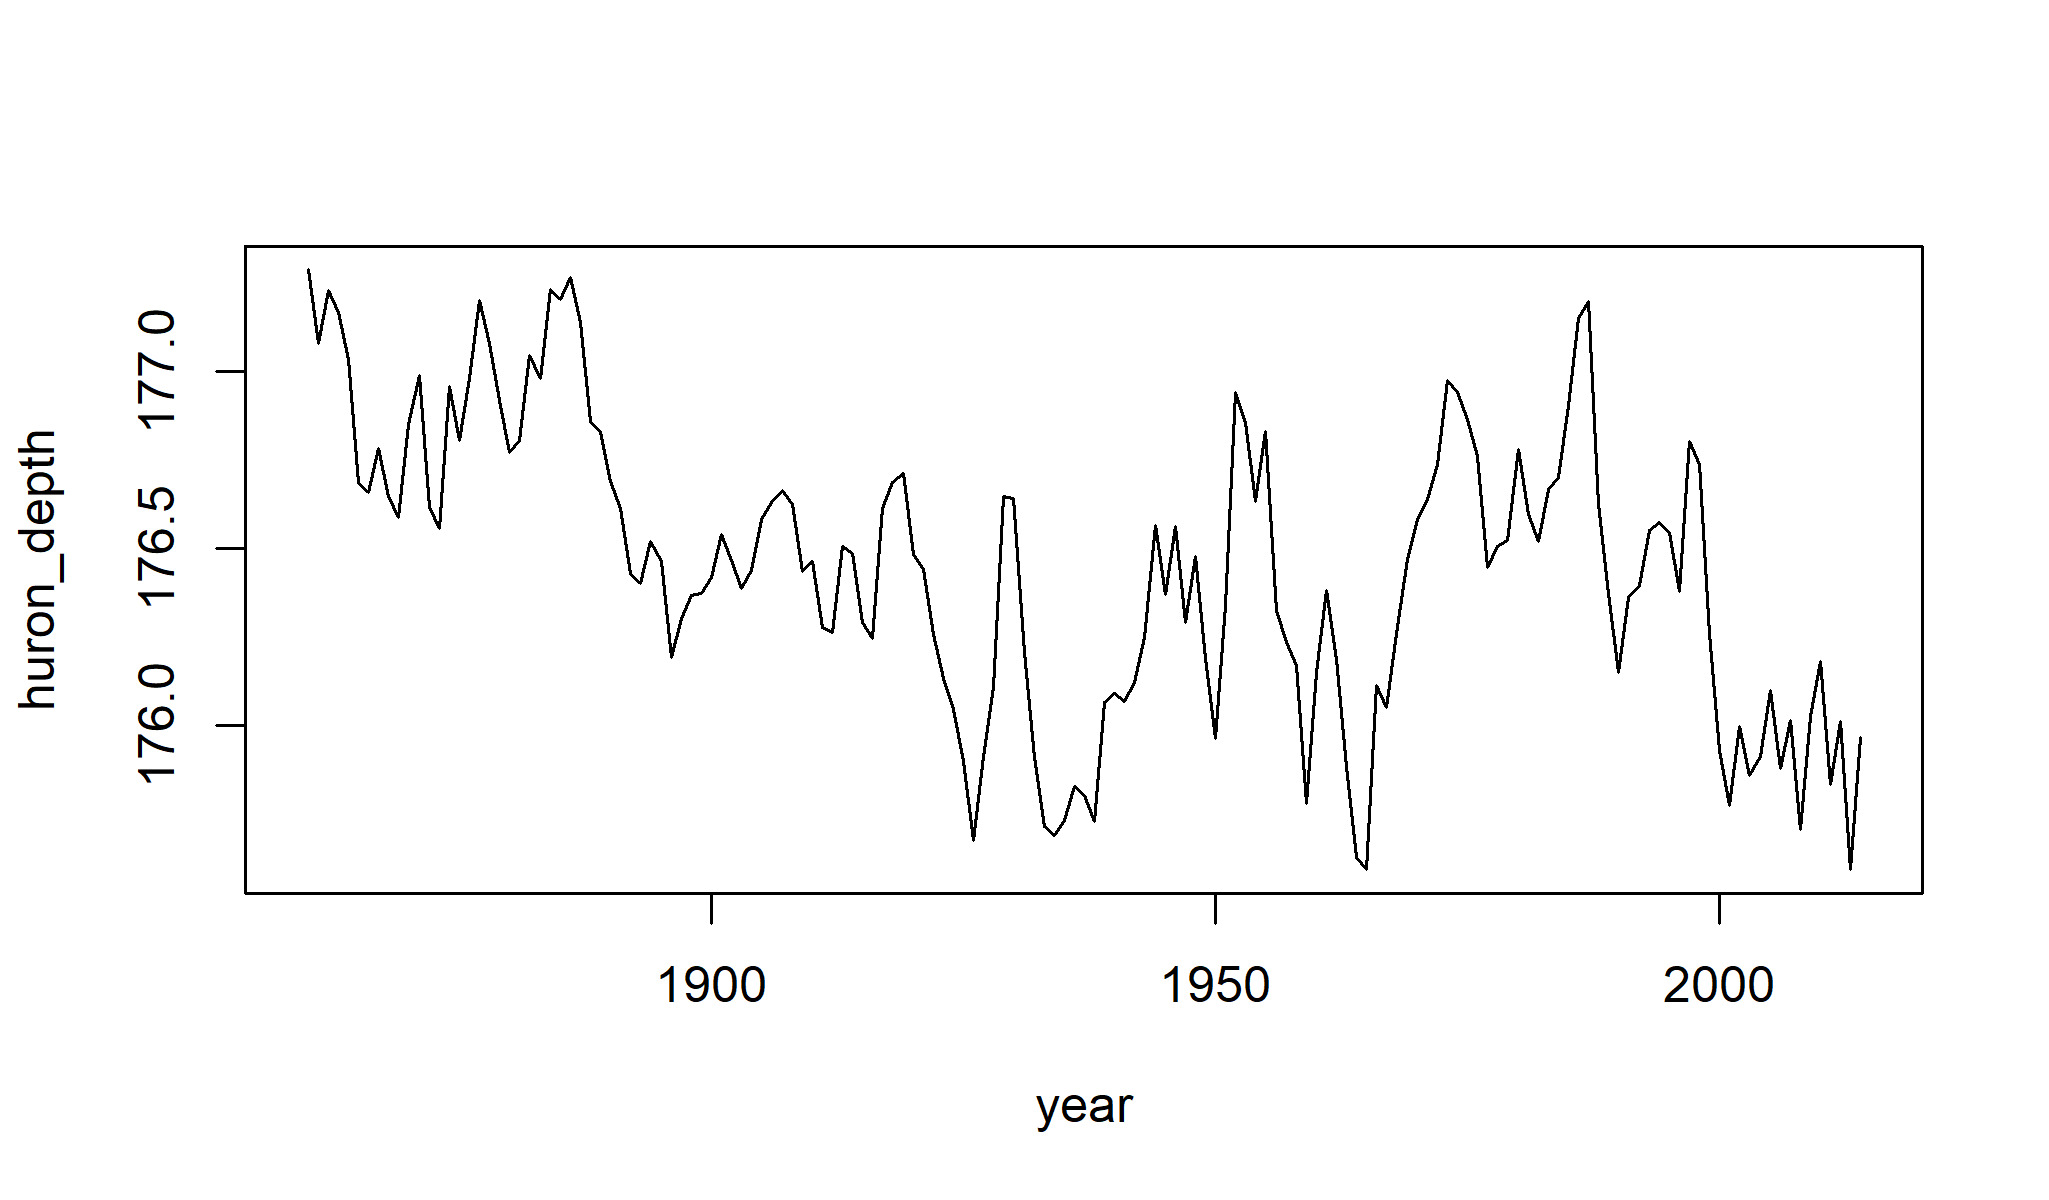
\includegraphics{figure/intro-select_annual-1} \end{center}

\begin{center}\rule{0.5\linewidth}{\linethickness}\end{center}

\begin{center}\rule{0.5\linewidth}{\linethickness}\end{center}

\subsubsection{Fitting an ARMA model}\label{fitting-an-arma-model}

\begin{itemize}
\item
  Later, we will consider hypotheses of trend. For now, let's start by
  fitting a stationary ARMA\((p,q)\) model under the null hypothesis
  that there is no trend. This hypothesis, which asserts that nothing
  has substantially changed in this system over the last 150 years, is
  not entirely unreasonable from looking at the data.
\item
  We seek to fit a stationary Gaussian ARMA(p,q) model with parameter
  vector \(\theta=(\ar_{1:p},\ma_{1:q},\mu,\sigma^2)\) given by
  \[ \ar(B)(Y_n-\mu) = \ma(B) \epsilon_n,\] where

  \begin{eqnarray}
  \mu &=& \E[Y_n]
  \\
  \ar(x)&=&1-\ar_1 x-\dots -\ar_px^p,
  \\ 
  \ma(x)&=&1+\ma_1 x+\dots +\ma_qx^q, 
  \\
  \epsilon_n&\sim&\mathrm{ iid }\, N[0,\sigma^2].
  \end{eqnarray}
\item
  We need to decide where to start in terms of values of \(p\) and
  \(q\). Let's tabulate some AIC values for a range of different choices
  of \(p\) and \(q\).
\item
  In the code below, note the use of \texttt{kable} for formatting HTML
  tables when using Rmarkdown. The \texttt{"\textless{}b\textgreater{}"}
  and \texttt{""\textless{}/b\textgreater{}"} tags in \texttt{dimnames}
  make the rownames boldface in HTML. By default, only column names are
  boldface in standard HTML.
\end{itemize}

\begin{Shaded}
\begin{Highlighting}[]
\NormalTok{aic_table <-}\StringTok{ }\ControlFlowTok{function}\NormalTok{(data,P,Q)\{}
\NormalTok{  table <-}\StringTok{ }\KeywordTok{matrix}\NormalTok{(}\OtherTok{NA}\NormalTok{,(P}\OperatorTok{+}\DecValTok{1}\NormalTok{),(Q}\OperatorTok{+}\DecValTok{1}\NormalTok{))}
  \ControlFlowTok{for}\NormalTok{(p }\ControlFlowTok{in} \DecValTok{0}\OperatorTok{:}\NormalTok{P) \{}
    \ControlFlowTok{for}\NormalTok{(q }\ControlFlowTok{in} \DecValTok{0}\OperatorTok{:}\NormalTok{Q) \{}
\NormalTok{       table[p}\OperatorTok{+}\DecValTok{1}\NormalTok{,q}\OperatorTok{+}\DecValTok{1}\NormalTok{] <-}\StringTok{ }\KeywordTok{arima}\NormalTok{(data,}\DataTypeTok{order=}\KeywordTok{c}\NormalTok{(p,}\DecValTok{0}\NormalTok{,q))}\OperatorTok{$}\NormalTok{aic}
\NormalTok{    \}}
\NormalTok{  \}}
  \KeywordTok{dimnames}\NormalTok{(table) <-}\StringTok{ }\KeywordTok{list}\NormalTok{(}\KeywordTok{paste}\NormalTok{(}\StringTok{"<b> AR"}\NormalTok{,}\DecValTok{0}\OperatorTok{:}\NormalTok{P, }\StringTok{"</b>"}\NormalTok{, }\DataTypeTok{sep=}\StringTok{""}\NormalTok{),}\KeywordTok{paste}\NormalTok{(}\StringTok{"MA"}\NormalTok{,}\DecValTok{0}\OperatorTok{:}\NormalTok{Q,}\DataTypeTok{sep=}\StringTok{""}\NormalTok{))}
\NormalTok{  table}
\NormalTok{\}}
\NormalTok{huron_aic_table <-}\StringTok{ }\KeywordTok{aic_table}\NormalTok{(huron_depth,}\DecValTok{4}\NormalTok{,}\DecValTok{5}\NormalTok{)}
\KeywordTok{require}\NormalTok{(knitr)}
\KeywordTok{kable}\NormalTok{(huron_aic_table,}\DataTypeTok{digits=}\DecValTok{2}\NormalTok{)}
\end{Highlighting}
\end{Shaded}

\begin{longtable}[]{@{}lrrrrrr@{}}
\toprule
& MA0 & MA1 & MA2 & MA3 & MA4 & MA5\tabularnewline
\midrule
\endhead
 AR0 & 166.75 & 46.60 & 7.28 & -14.97 & -18.64 & -26.09\tabularnewline
 AR1 & -38.00 & -37.41 & -35.46 & -33.82 & -34.13 &
-32.20\tabularnewline
 AR2 & -37.33 & -38.43 & -36.90 & -34.93 & -34.35 &
-33.08\tabularnewline
 AR3 & -35.52 & -35.17 & -32.71 & -31.38 & -33.21 &
-32.98\tabularnewline
 AR4 & -33.94 & -34.91 & -34.43 & -37.48 & -31.31 &
-30.90\tabularnewline
\bottomrule
\end{longtable}

\begin{center}\rule{0.5\linewidth}{\linethickness}\end{center}

\begin{center}\rule{0.5\linewidth}{\linethickness}\end{center}

\subsubsection{Question: What do we learn by interpreting the results in
the above table of AIC
values?}\label{question-what-do-we-learn-by-interpreting-the-results-in-the-above-table-of-aic-values}

\subsubsection{Question: In what ways might we have to be careful not to
over-interpret the results of this
table?}\label{question-in-what-ways-might-we-have-to-be-careful-not-to-over-interpret-the-results-of-this-table}

\begin{center}\rule{0.5\linewidth}{\linethickness}\end{center}

\begin{center}\rule{0.5\linewidth}{\linethickness}\end{center}

\begin{itemize}
\tightlist
\item
  Let's fit the ARMA(2,1) model recommended by consideration of AIC.
\end{itemize}

\begin{Shaded}
\begin{Highlighting}[]
\NormalTok{huron_arma21 <-}\StringTok{ }\KeywordTok{arima}\NormalTok{(huron_depth,}\DataTypeTok{order=}\KeywordTok{c}\NormalTok{(}\DecValTok{2}\NormalTok{,}\DecValTok{0}\NormalTok{,}\DecValTok{1}\NormalTok{))}
\NormalTok{huron_arma21}
\end{Highlighting}
\end{Shaded}

\begin{verbatim}
## 
## Call:
## arima(x = huron_depth, order = c(2, 0, 1))
## 
## Coefficients:
##           ar1     ar2     ma1  intercept
##       -0.0525  0.7910  1.0000   176.4603
## s.e.   0.0522  0.0526  0.0242     0.1210
## 
## sigma^2 estimated as 0.04188:  log likelihood = 24.21,  aic = -38.43
\end{verbatim}

\begin{itemize}
\tightlist
\item
  We can examine the roots of the AR polynomial,
\end{itemize}

\begin{Shaded}
\begin{Highlighting}[]
\NormalTok{AR_roots <-}\StringTok{ }\KeywordTok{polyroot}\NormalTok{(}\KeywordTok{c}\NormalTok{(}\DecValTok{1}\NormalTok{,}\OperatorTok{-}\KeywordTok{coef}\NormalTok{(huron_arma21)[}\KeywordTok{c}\NormalTok{(}\StringTok{"ar1"}\NormalTok{,}\StringTok{"ar2"}\NormalTok{)]))}
\NormalTok{AR_roots}
\end{Highlighting}
\end{Shaded}

\begin{verbatim}
## [1]  1.158083-0i -1.091668+0i
\end{verbatim}

\begin{itemize}
\item
  These are just outside the unit circle, suggesting we have a
  stationary causal fitted ARMA.
\item
  However, the MA root is -1, showing that the fitted model is at the
  threshold of non-invertibility.
\item
  Is this non-invertibility a problem? Let's investigate a little, using
  profile and bootstrap methods. The claimed standard error on the MA1
  coefficient, from the Fisher information approach used by
  \texttt{arima} is small.
\item
  First, we can see if the approximate confidence interval constructed
  using profile likelihood is in agreement with the approximate
  confidence interval constructed using the observed Fisher information.
\item
  To do this, we need to maximize the ARMA likelihood while fixing the
  MA1 coefficient at a range of values. This can be done using
  \texttt{arima} as follows. Note that the \texttt{fixed} argument
  expects a vector of length \(p+q+1\) corresponding to a concatenated
  vector \((\ar_{1:p},\ma_{1:q}, \mu)\). Somehow, the Gaussian white
  noise variance, \(\sigma^2\), is not included in this representation.
  Parameters with \texttt{NA} entries in \texttt{fixed} are estimated.
\end{itemize}

\begin{Shaded}
\begin{Highlighting}[]
\NormalTok{K <-}\StringTok{ }\DecValTok{500}
\NormalTok{ma1 <-}\StringTok{ }\KeywordTok{seq}\NormalTok{(}\DataTypeTok{from=}\FloatTok{0.2}\NormalTok{,}\DataTypeTok{to=}\FloatTok{1.1}\NormalTok{,}\DataTypeTok{length=}\NormalTok{K)}
\NormalTok{profile_loglik <-}\StringTok{ }\KeywordTok{rep}\NormalTok{(}\OtherTok{NA}\NormalTok{,K)}
\ControlFlowTok{for}\NormalTok{(k }\ControlFlowTok{in} \DecValTok{1}\OperatorTok{:}\NormalTok{K)\{}
\NormalTok{   profile_loglik[k] <-}\StringTok{ }\KeywordTok{logLik}\NormalTok{(}\KeywordTok{arima}\NormalTok{(huron_depth,}\DataTypeTok{order=}\KeywordTok{c}\NormalTok{(}\DecValTok{2}\NormalTok{,}\DecValTok{0}\NormalTok{,}\DecValTok{1}\NormalTok{),}
      \DataTypeTok{fixed=}\KeywordTok{c}\NormalTok{(}\OtherTok{NA}\NormalTok{,}\OtherTok{NA}\NormalTok{,ma1[k],}\OtherTok{NA}\NormalTok{)))}
\NormalTok{\}}
\KeywordTok{plot}\NormalTok{(profile_loglik}\OperatorTok{~}\NormalTok{ma1,}\DataTypeTok{ty=}\StringTok{"l"}\NormalTok{)}
\end{Highlighting}
\end{Shaded}

\begin{center}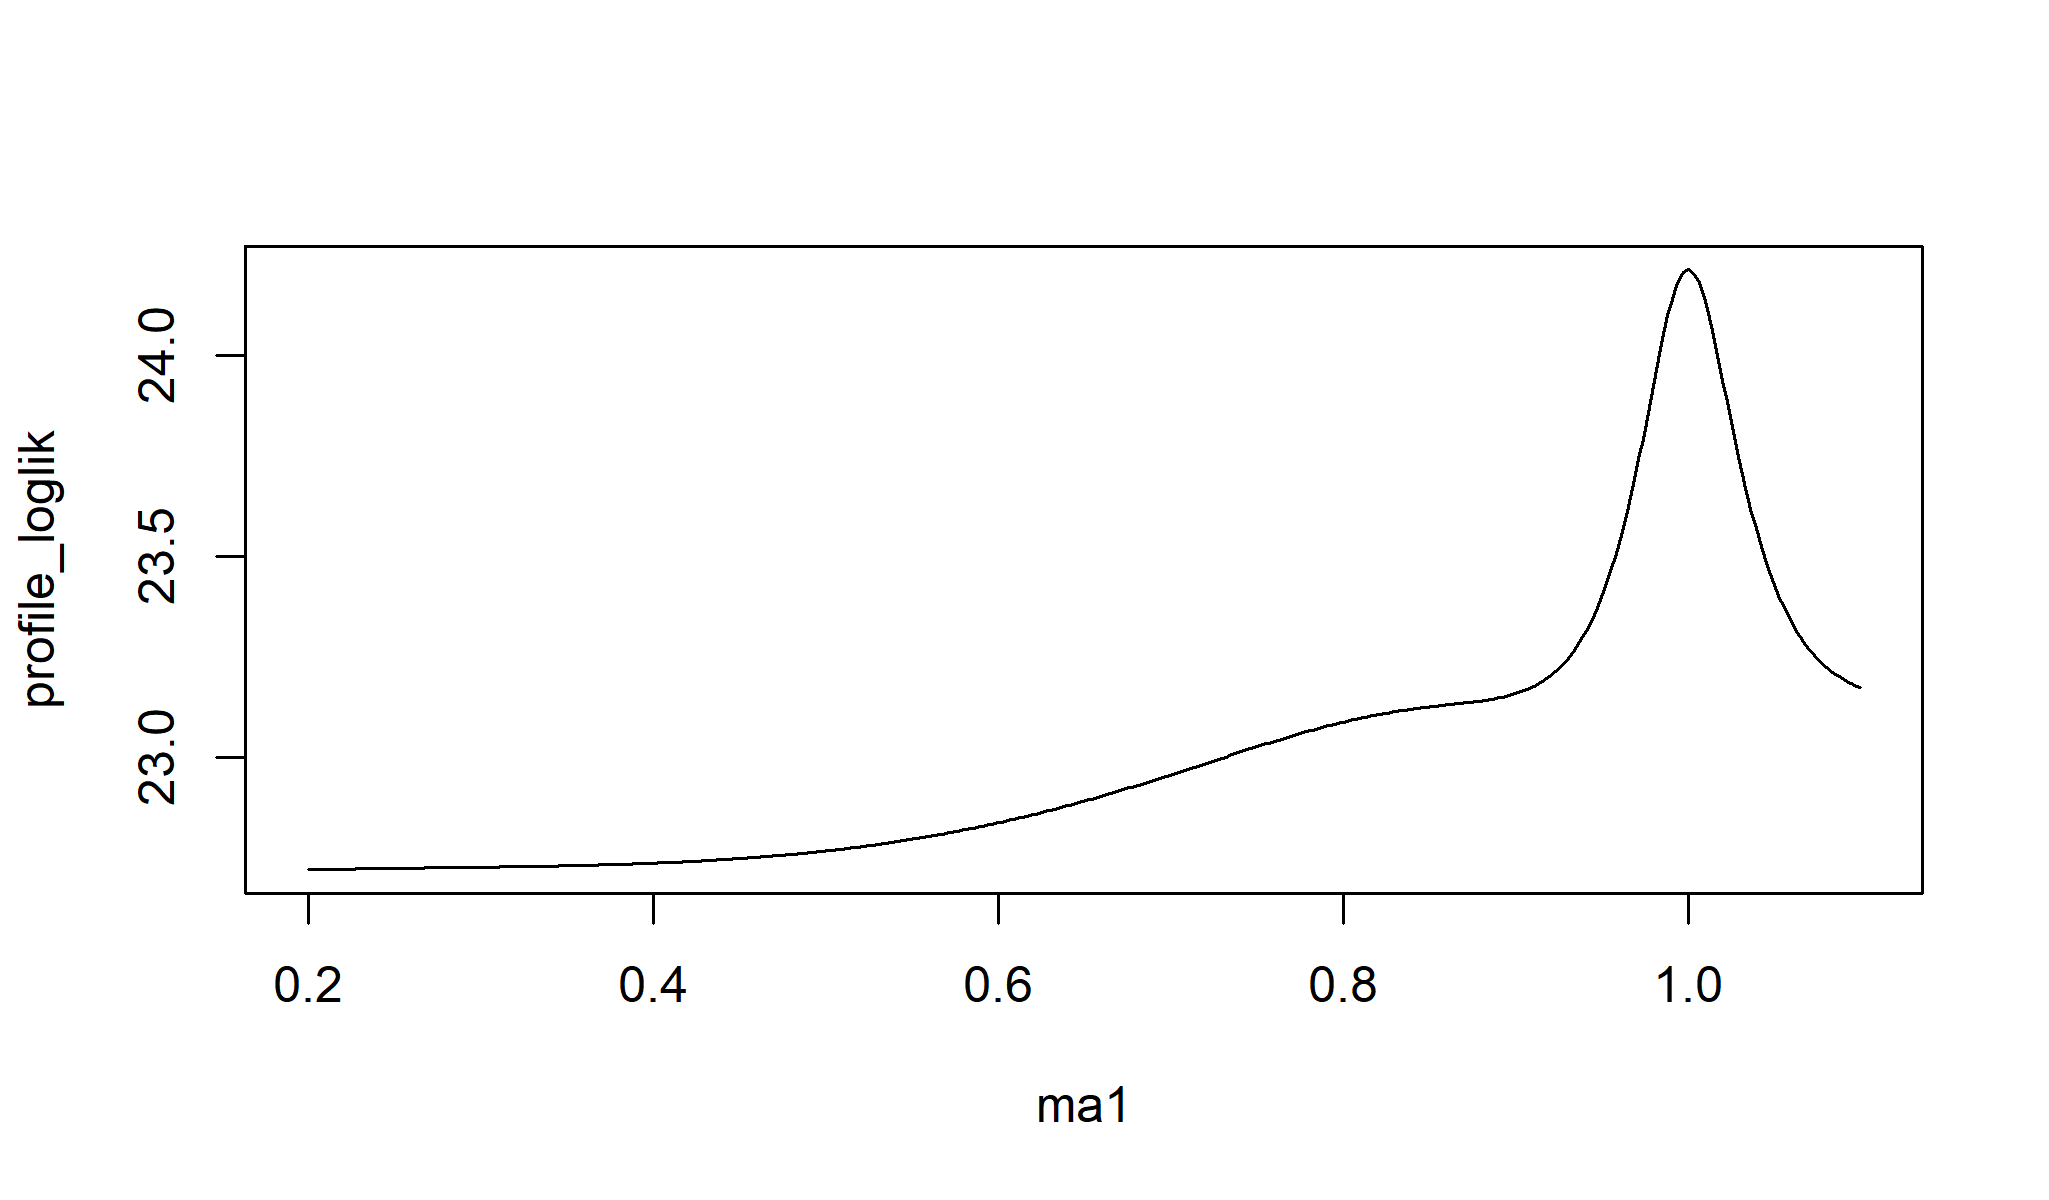
\includegraphics{figure/intro-huron_profile-1} \end{center}

\subsubsection{\texorpdfstring{Question: Interpret the profile
likelihood plot for
\(\ma_1\).}{Question: Interpret the profile likelihood plot for \textbackslash{}ma\_1.}}\label{question-interpret-the-profile-likelihood-plot-for-ma_1.}

\begin{itemize}
\item
  What do you conclude about the Fisher information confidence interval
  proposed by \texttt{arima}?
\item
  When do you think the Fisher information confidence interval may be
  reliable?
\item
  Is this profile likelihood plot, and its statistical interpretation,
  reliable? How do you support your opinion on this?
\end{itemize}

\begin{center}\rule{0.5\linewidth}{\linethickness}\end{center}

\begin{center}\rule{0.5\linewidth}{\linethickness}\end{center}

\begin{itemize}
\tightlist
\item
  Let's do a simulation study
\end{itemize}

\begin{Shaded}
\begin{Highlighting}[]
\KeywordTok{set.seed}\NormalTok{(}\DecValTok{57892330}\NormalTok{)}
\NormalTok{J <-}\StringTok{ }\DecValTok{1000}
\NormalTok{params <-}\StringTok{ }\KeywordTok{coef}\NormalTok{(huron_arma21)}
\NormalTok{ar <-}\StringTok{ }\NormalTok{params[}\KeywordTok{grep}\NormalTok{(}\StringTok{"^ar"}\NormalTok{,}\KeywordTok{names}\NormalTok{(params))]}
\NormalTok{ma <-}\StringTok{ }\NormalTok{params[}\KeywordTok{grep}\NormalTok{(}\StringTok{"^ma"}\NormalTok{,}\KeywordTok{names}\NormalTok{(params))]}
\NormalTok{intercept <-}\StringTok{ }\NormalTok{params[}\StringTok{"intercept"}\NormalTok{]}
\NormalTok{sigma <-}\StringTok{ }\KeywordTok{sqrt}\NormalTok{(huron_arma21}\OperatorTok{$}\NormalTok{sigma2)}
\NormalTok{theta <-}\StringTok{ }\KeywordTok{matrix}\NormalTok{(}\OtherTok{NA}\NormalTok{,}\DataTypeTok{nrow=}\NormalTok{J,}\DataTypeTok{ncol=}\KeywordTok{length}\NormalTok{(params),}\DataTypeTok{dimnames=}\KeywordTok{list}\NormalTok{(}\OtherTok{NULL}\NormalTok{,}\KeywordTok{names}\NormalTok{(params)))}
\ControlFlowTok{for}\NormalTok{(j }\ControlFlowTok{in} \DecValTok{1}\OperatorTok{:}\NormalTok{J)\{}
\NormalTok{   Y_j <-}\StringTok{ }\KeywordTok{arima.sim}\NormalTok{(}
      \KeywordTok{list}\NormalTok{(}\DataTypeTok{ar=}\NormalTok{ar,}\DataTypeTok{ma=}\NormalTok{ma),}
      \DataTypeTok{n=}\KeywordTok{length}\NormalTok{(huron_depth),}
      \DataTypeTok{sd=}\NormalTok{sigma}
\NormalTok{   )}\OperatorTok{+}\NormalTok{intercept}
\NormalTok{   theta[j,] <-}\StringTok{ }\KeywordTok{coef}\NormalTok{(}\KeywordTok{arima}\NormalTok{(Y_j,}\DataTypeTok{order=}\KeywordTok{c}\NormalTok{(}\DecValTok{2}\NormalTok{,}\DecValTok{0}\NormalTok{,}\DecValTok{1}\NormalTok{)))}
\NormalTok{\}}
\KeywordTok{hist}\NormalTok{(theta[,}\StringTok{"ma1"}\NormalTok{],}\DataTypeTok{freq=}\OtherTok{FALSE}\NormalTok{) }
\end{Highlighting}
\end{Shaded}

\begin{center}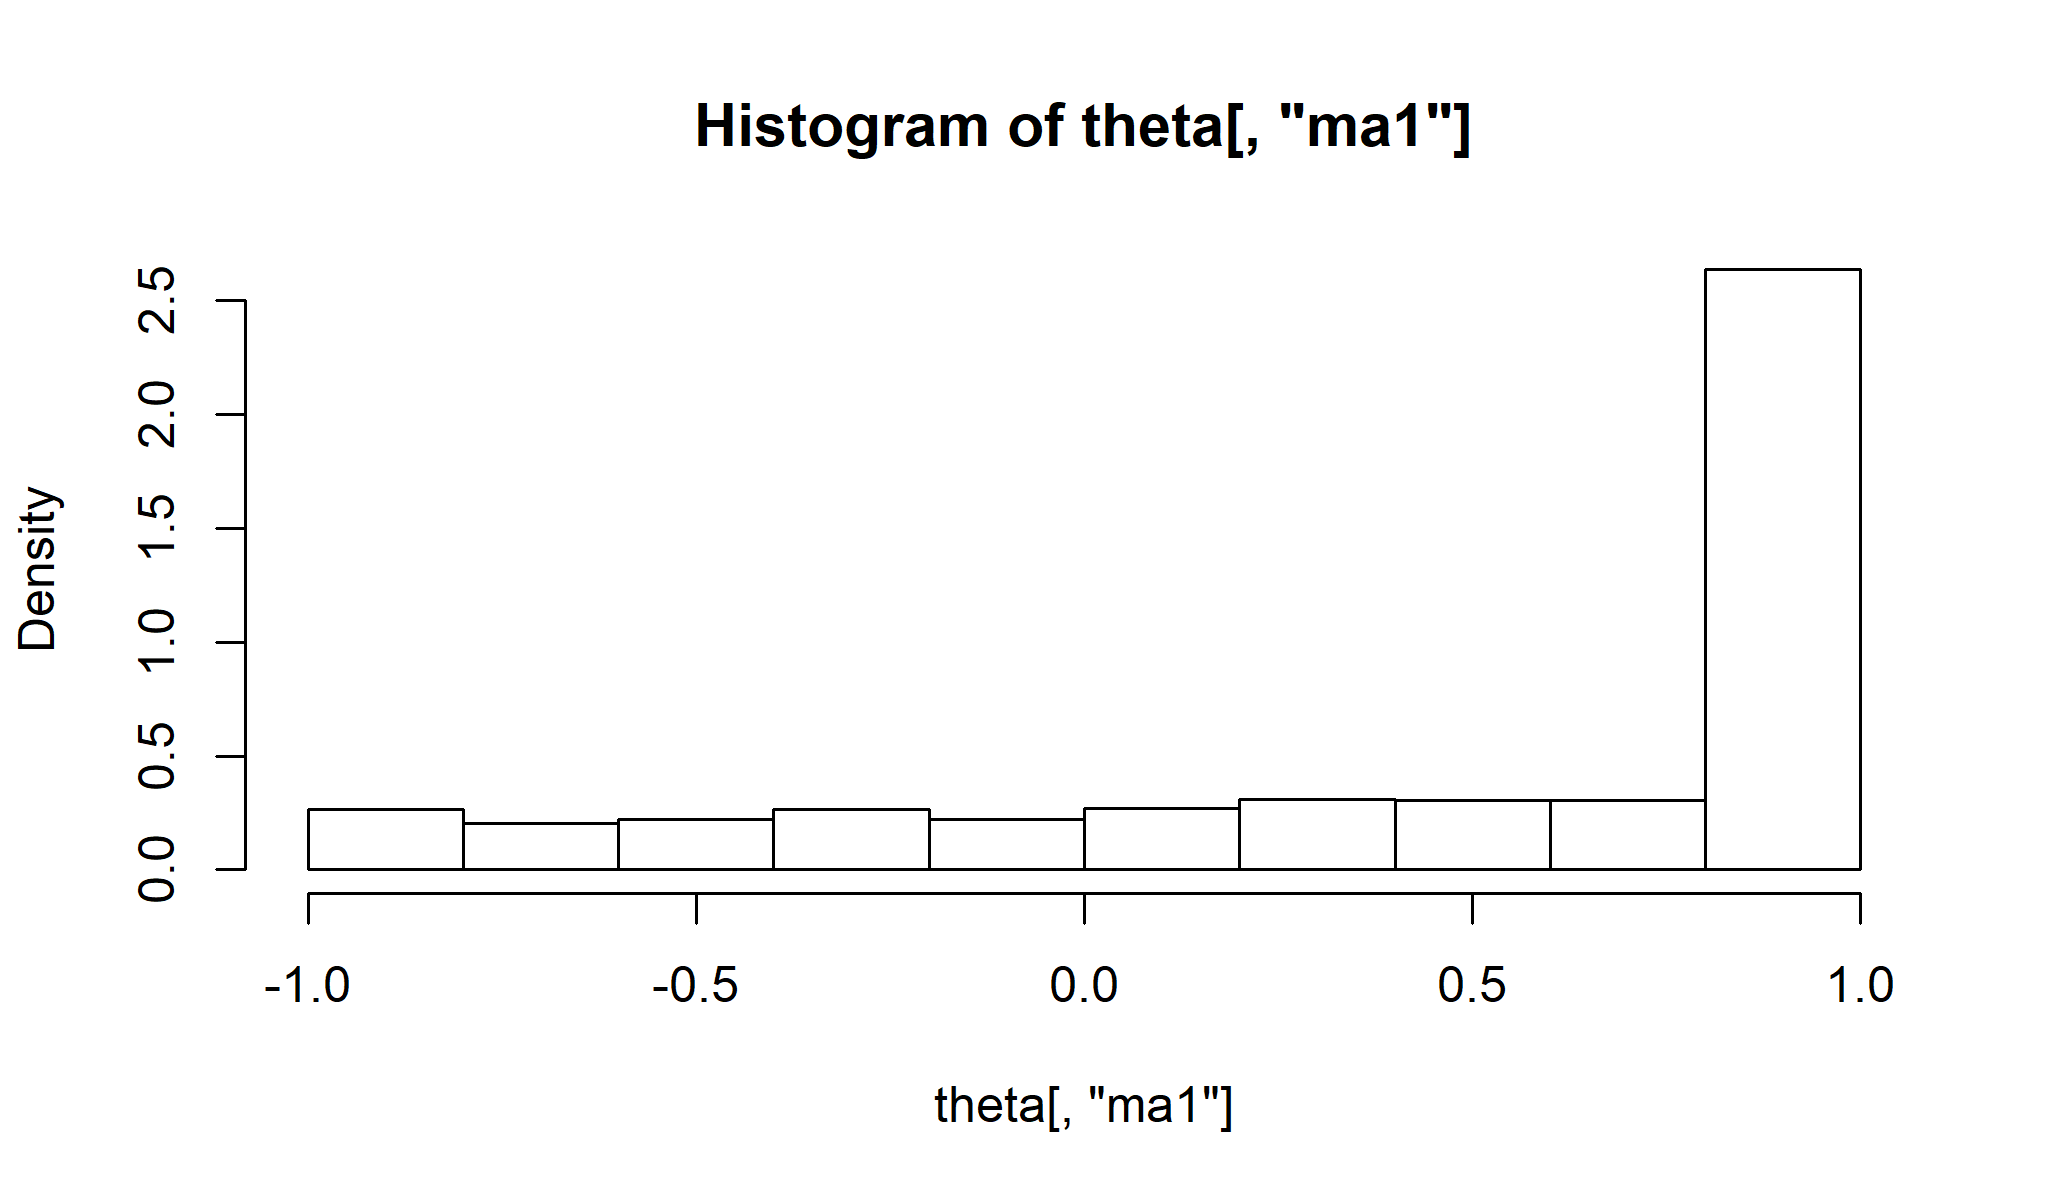
\includegraphics{figure/intro-simA-1} \end{center}

\begin{itemize}
\item
  This seems consistent with the profile likelihood plot.
\item
  A density plot shows this similarity even more clearly.
\end{itemize}

\begin{Shaded}
\begin{Highlighting}[]
\KeywordTok{plot}\NormalTok{(}\KeywordTok{density}\NormalTok{(theta[,}\StringTok{"ma1"}\NormalTok{],}\DataTypeTok{bw=}\FloatTok{0.05}\NormalTok{))}
\end{Highlighting}
\end{Shaded}

\begin{center}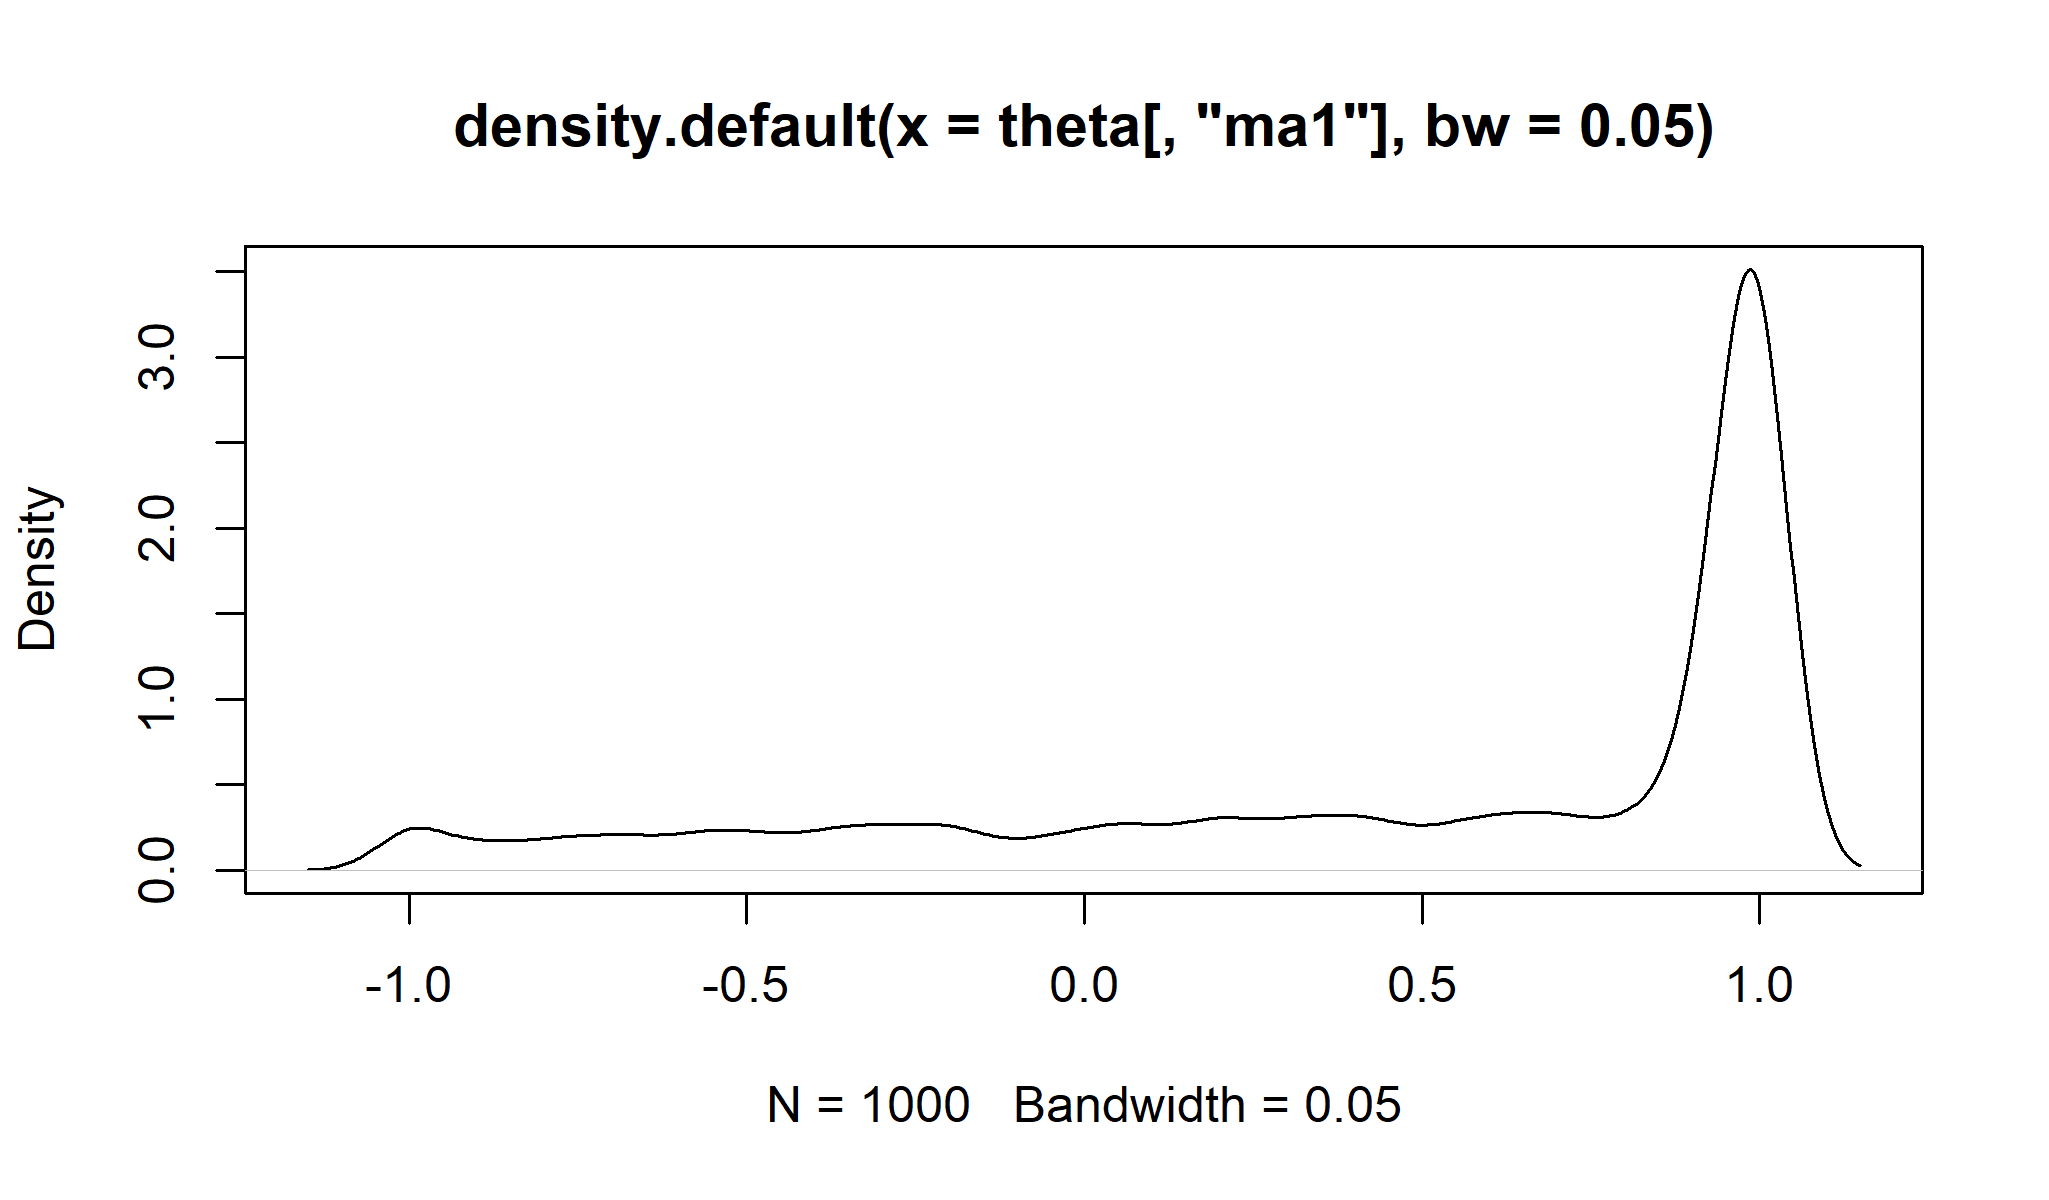
\includegraphics{figure/intro-density-1} \end{center}

\begin{itemize}
\item
  Here, I'm showing the raw plot for instructional purposes. For a
  report, one should improve the default axis labels and title.
\item
  Note that \texttt{arima} transforms the model to invertibility. Thus,
  the estimated value of \(\theta_1\) can only fall in the interval
  \((-1,1)\) but can be arbitrarily close to \(-1\) or \(1\).
\end{itemize}

\begin{Shaded}
\begin{Highlighting}[]
\KeywordTok{range}\NormalTok{(theta[,}\StringTok{"ma1"}\NormalTok{])}
\end{Highlighting}
\end{Shaded}

\begin{verbatim}
## [1] -1  1
\end{verbatim}

\begin{verbatim}
+ Estimated densities outside $[-1,1]$ are artifacts of the density estimation procedure. 

+ How would you refine this procedure to get a density estimate respecting the range of the parameter estimation procedure?
\end{verbatim}

\begin{itemize}
\item
  To understand what is going on better, it is helpful to do another
  simulation study for which we fit ARMA(2,1) when the true model is
  AR(1).
\item
  When doing simulation studies, it is helpful to use multicore
  computing, which most of us have on our machines nowadays.
\item
  A basic approach to multicore statistical computing is to tell R you
  want it to look for available processors, using the
  \texttt{doParallel} package.
\end{itemize}

\begin{Shaded}
\begin{Highlighting}[]
\KeywordTok{require}\NormalTok{(doParallel)}
\KeywordTok{registerDoParallel}\NormalTok{()}
\end{Highlighting}
\end{Shaded}

\begin{itemize}
\tightlist
\item
  Then, we can use \texttt{foreach} to carry out a parallel \texttt{for}
  loop where jobs are sent to different processors.
\end{itemize}

\begin{Shaded}
\begin{Highlighting}[]
\NormalTok{J <-}\StringTok{ }\DecValTok{1000}
\NormalTok{huron_ar1 <-}\StringTok{ }\KeywordTok{arima}\NormalTok{(huron_depth,}\DataTypeTok{order=}\KeywordTok{c}\NormalTok{(}\DecValTok{1}\NormalTok{,}\DecValTok{0}\NormalTok{,}\DecValTok{0}\NormalTok{),}\DataTypeTok{method=}\StringTok{'ML'}\NormalTok{)}
\NormalTok{params <-}\StringTok{ }\KeywordTok{coef}\NormalTok{(huron_ar1)}
\NormalTok{ar <-}\StringTok{ }\NormalTok{params[}\KeywordTok{grep}\NormalTok{(}\StringTok{"^ar"}\NormalTok{,}\KeywordTok{names}\NormalTok{(params))]}
\NormalTok{intercept <-}\StringTok{ }\NormalTok{params[}\StringTok{"intercept"}\NormalTok{]}
\NormalTok{sigma <-}\StringTok{ }\KeywordTok{sqrt}\NormalTok{(huron_ar1}\OperatorTok{$}\NormalTok{sigma2)}
\NormalTok{t1 <-}\StringTok{ }\KeywordTok{system.time}\NormalTok{(}
\NormalTok{  huron_sim <-}\StringTok{ }\KeywordTok{foreach}\NormalTok{(}\DataTypeTok{j=}\DecValTok{1}\OperatorTok{:}\NormalTok{J) }\OperatorTok\StringTok{ }\NormalTok{\{}
\NormalTok{     Y_j <-}\StringTok{ }\KeywordTok{arima.sim}\NormalTok{(}\KeywordTok{list}\NormalTok{(}\DataTypeTok{ar=}\NormalTok{ar),}\DataTypeTok{n=}\KeywordTok{length}\NormalTok{(huron_depth),}\DataTypeTok{sd=}\NormalTok{sigma)}\OperatorTok{+}\NormalTok{intercept}
     \KeywordTok{try}\NormalTok{(}\KeywordTok{coef}\NormalTok{(}\KeywordTok{arima}\NormalTok{(Y_j,}\DataTypeTok{order=}\KeywordTok{c}\NormalTok{(}\DecValTok{2}\NormalTok{,}\DecValTok{0}\NormalTok{,}\DecValTok{1}\NormalTok{),}\DataTypeTok{method=}\StringTok{'ML'}\NormalTok{)))}
\NormalTok{  \}}
\NormalTok{) }
\end{Highlighting}
\end{Shaded}

\begin{itemize}
\tightlist
\item
  Some of these \texttt{arima} calls did not successfully produce
  parameter estimates. The \texttt{try} function lets the simulation
  proceed despite these errors. Let's see how many of them fail:
\end{itemize}

\begin{Shaded}
\begin{Highlighting}[]
\KeywordTok{sum}\NormalTok{(}\KeywordTok{sapply}\NormalTok{(huron_sim, }\ControlFlowTok{function}\NormalTok{(x) }\KeywordTok{inherits}\NormalTok{(x,}\StringTok{"try-error"}\NormalTok{))) }
\end{Highlighting}
\end{Shaded}

\begin{verbatim}
## [1] 0
\end{verbatim}

\begin{itemize}
\tightlist
\item
  Now, for the remaining ones, we can look at the resulting estimates of
  the MA1 component:
\end{itemize}

\begin{Shaded}
\begin{Highlighting}[]
\NormalTok{ma1 <-}\StringTok{ }\KeywordTok{unlist}\NormalTok{(}\KeywordTok{lapply}\NormalTok{(huron_sim,}\ControlFlowTok{function}\NormalTok{(x) }\ControlFlowTok{if}\NormalTok{(}\OperatorTok{!}\KeywordTok{inherits}\NormalTok{(x,}\StringTok{"try-error"}\NormalTok{))x[}\StringTok{"ma1"}\NormalTok{] }\ControlFlowTok{else} \OtherTok{NULL}\NormalTok{ ))}
\KeywordTok{hist}\NormalTok{(ma1,}\DataTypeTok{breaks=}\DecValTok{50}\NormalTok{)  }
\end{Highlighting}
\end{Shaded}

\begin{center}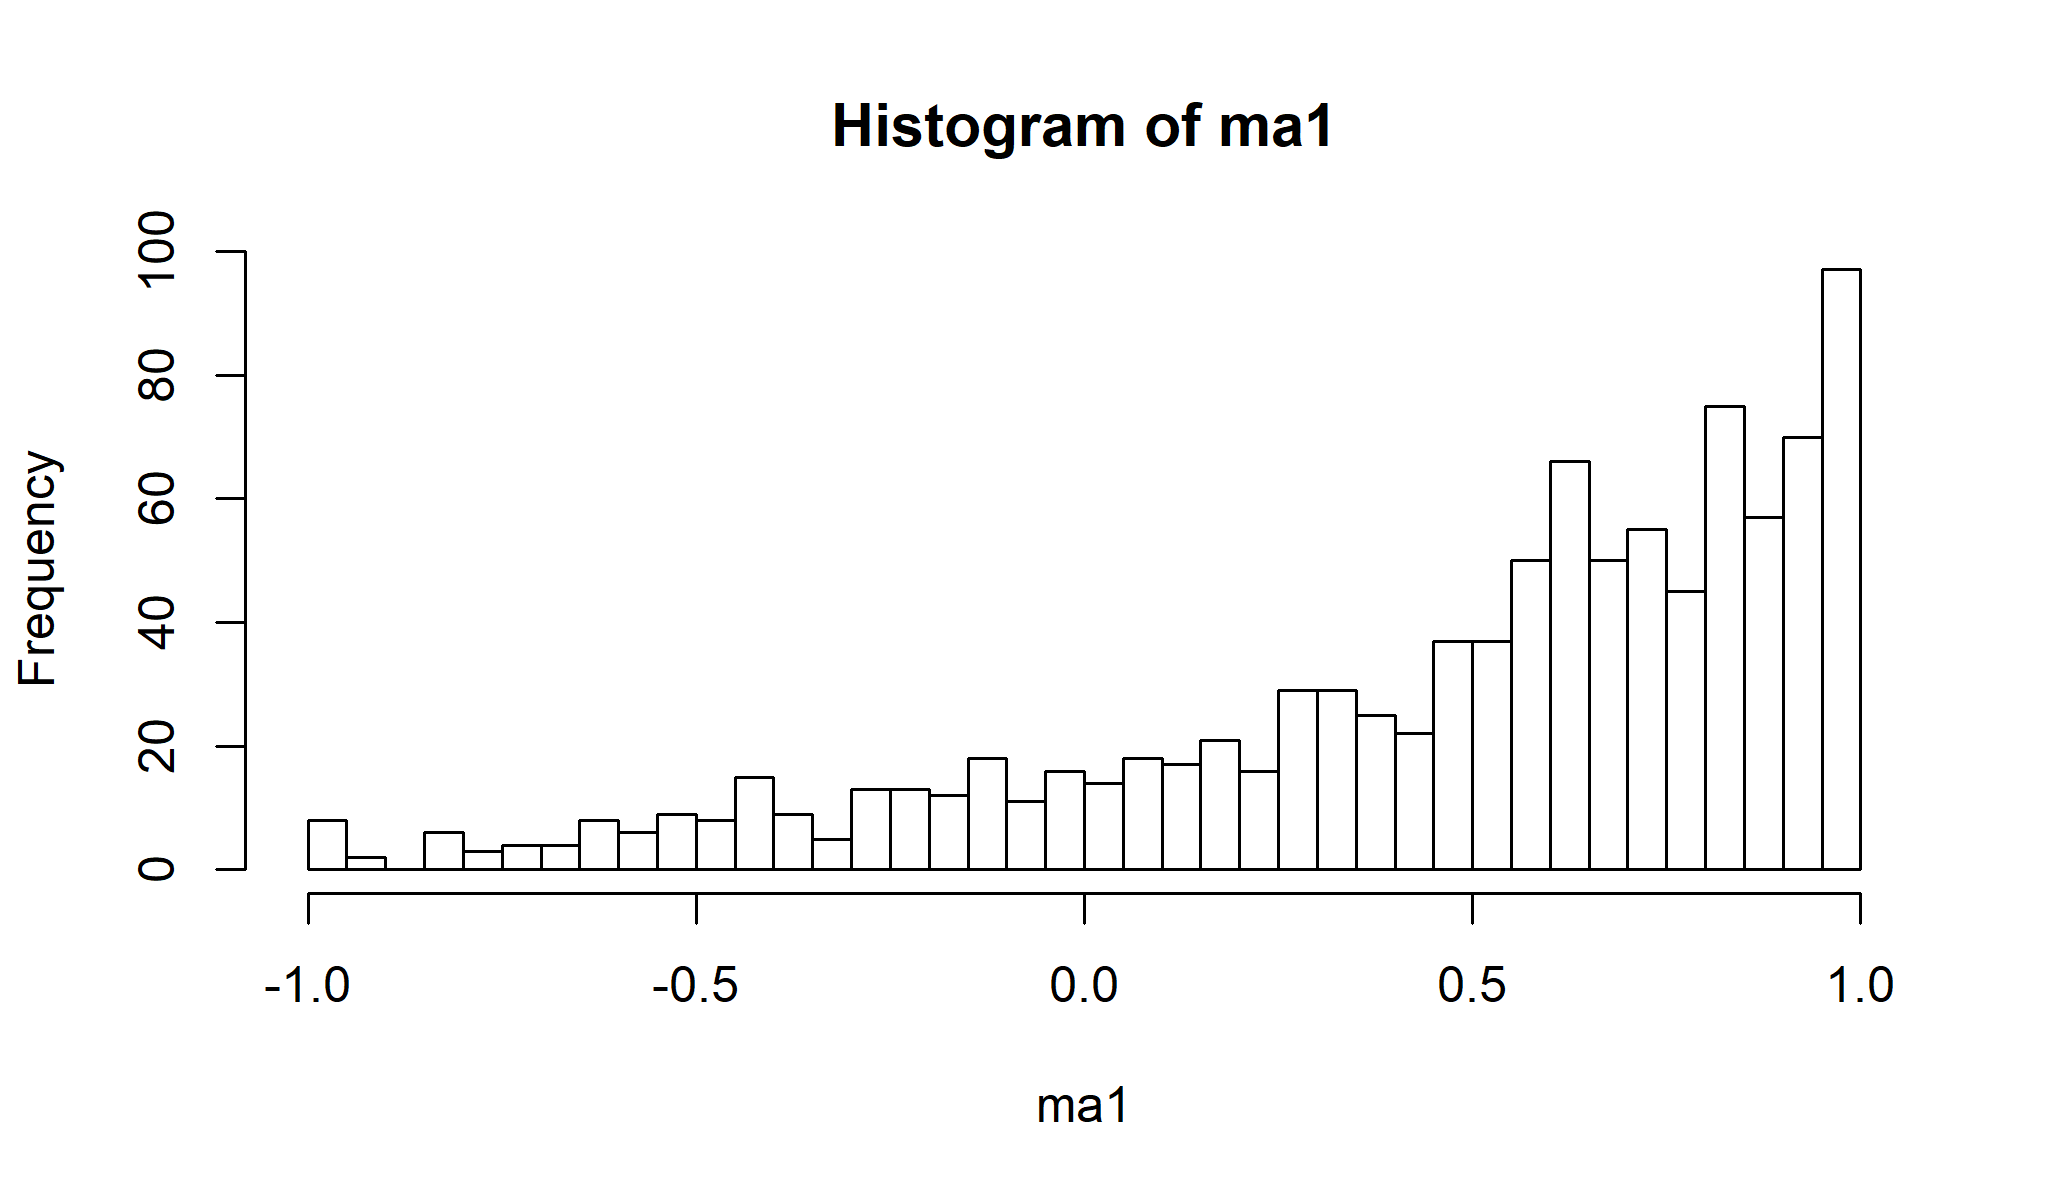
\includegraphics{figure/intro-histB-1} \end{center}

\begin{itemize}
\item
  When the true model is AR1 and we fit ARMA(2,1), it seems that we
  often obtain a model with estimated MA1 coefficient on the boundary of
  invertibility.
\item
  It is clear from this that we cannot reject an AR1 hypothesis, even
  though the Fisher information based analysis appears to give strong
  evidence that the data should be modeled with a nonzero MA1
  coefficient.
\item
  It may be sensible to avoid fitted models too close to the boundary of
  invertibility. This is a reason not to blindly accept whatever model
  AIC might suggest.
\end{itemize}

\begin{center}\rule{0.5\linewidth}{\linethickness}\end{center}

\begin{center}\rule{0.5\linewidth}{\linethickness}\end{center}

\subsubsection{Question: what else could we look for to help diagnose,
and understand, this kind of model fitting
problem?}\label{question-what-else-could-we-look-for-to-help-diagnose-and-understand-this-kind-of-model-fitting-problem}

\begin{itemize}
\tightlist
\item
  Hint: pay some more attention to the roots of the fitted ARMA(2,1)
  model.
\end{itemize}

\begin{center}\rule{0.5\linewidth}{\linethickness}\end{center}

\begin{center}\rule{0.5\linewidth}{\linethickness}\end{center}

\subsection{Assessing the numerical correctness of evaluation and
maximization of the likelihood
function}\label{assessing-the-numerical-correctness-of-evaluation-and-maximization-of-the-likelihood-function}

\begin{itemize}
\item
  We can probably suppose that \texttt{arima} has negligible numerical
  error in evaluating the likelihood.

  \begin{itemize}
  \item
    Likelihood evaluation is a linear algebra computation which should
    be numerically stable away from singularities.
  \item
    Possibly, numerical problems could arise for models very close to
    reducibility (canceling AR and MA roots).
  \end{itemize}
\item
  Numerical optimization is more problematic.

  \begin{itemize}
  \item
    \texttt{arima} calls the general purpose optimization routine
    \texttt{optim}.
  \item
    We know the likelihood surface can be multimodal and have nonlinear
    ridges; both these are consequences of the possibility of
    reducibility or near reducibility (AR and MA roots which almost
    cancel).
  \item
    No optimization procedure is reliable for maximizing awkward,
    non-convex functions.
  \item
    Evidence for imperfect maximization (assuming negligible likelihood
    evaluation error) can be found in the above AIC table, reproduced
    here:
  \end{itemize}
\end{itemize}

\begin{center}\rule{0.5\linewidth}{\linethickness}\end{center}

\begin{longtable}[]{@{}lrrrrrr@{}}
\toprule
& MA0 & MA1 & MA2 & MA3 & MA4 & MA5\tabularnewline
\midrule
\endhead
 AR0 & 166.75 & 46.60 & 7.28 & -14.97 & -18.64 & -26.09\tabularnewline
 AR1 & -38.00 & -37.41 & -35.46 & -33.82 & -34.13 &
-32.20\tabularnewline
 AR2 & -37.33 & -38.43 & -36.90 & -34.93 & -34.35 &
-33.08\tabularnewline
 AR3 & -35.52 & -35.17 & -32.71 & -31.38 & -33.21 &
-32.98\tabularnewline
 AR4 & -33.94 & -34.91 & -34.43 & -37.48 & -31.31 &
-30.90\tabularnewline
\bottomrule
\end{longtable}

\begin{center}\rule{0.5\linewidth}{\linethickness}\end{center}

\begin{center}\rule{0.5\linewidth}{\linethickness}\end{center}

\subsubsection{Question: How is this table inconsistent with perfect
maximization?}\label{question-how-is-this-table-inconsistent-with-perfect-maximization}

\begin{itemize}
\item
  Here are two hints:

  \begin{itemize}
  \item
    Recall that, for nested hypotheses
    \(H^{\langle 0\rangle}\subset H^{\langle 1\rangle}\), the likelihood
    maximized over \(H^{\langle 1\rangle}\) cannot be less than the
    likelihood maximized over \(H^{\langle 0\rangle}\).
  \item
    Recall also the definition of AIC, AIC = -2\(\times\) maximized log
    likelihood \(+\) 2\(\times\) number of parameters
  \end{itemize}
\end{itemize}

\begin{center}\rule{0.5\linewidth}{\linethickness}\end{center}

\begin{center}\rule{0.5\linewidth}{\linethickness}\end{center}


\end{document}
